\section{State-of-the-art protein language modeling}
\label{nlp}
It is intuitive to represent a protein as a sequence of letters with each letter corresponding to an amino acid. As with natural languages, we can find common elements between naturally evolved proteins. Noticeable patterns reoccurring in multiple (related) protein sequences are highly likely to be biologically relevant. These motifs and domains are essential to many biological processes and can easily be represented as words, phrases or sentences of amino acids in a language model perspective. This is why researchers are taking inspiration from the recent successes of natural language processing (NLP) and applying this to a biological context. NLP is a branch of artificial intelligence (AI) concerning itself with creating the ability for computers to learn and understand human languages by using statistical, machine learning and in recent years deep learning models~\cite{Ofer}. Common tasks in NLP include part-of-speech tagging (grouping words based on their function in a sentence), named entity recognition (recognizing specific entities in a sentence such as locations, persons, dates etc.) and natural language generation (letter/word prediction).

As with protein modeling, applying labels to millions of natural language containing web pages, articles, journals etc.\ is a labor-intensive procedure and thus state-of-the-art NLP models use a form of \textit{self-supervised learning}, a form of unsupervised learning in which the context of the text is learned to fill in missing words, predict the next word in a sentence etc. during the training as shown in figure~\ref{fig:ofer}. Well-known NLP methods of this kind include bi-directional long-short term recurrent neural networks (biLSTMs) such as ELMo~\cite{elmo} and more recently transformers such as Google's BERT~\cite{bert} and OpenAI's GPT-3~\cite{gpt3}. Despite the simplicity of these tasks, it is found to develop interesting capabilities as the scale of the model increases together with very little training on a specific task, now mostly referred to as \textit{few-shot learning}.

\begin{figure}[h]
    \centering
    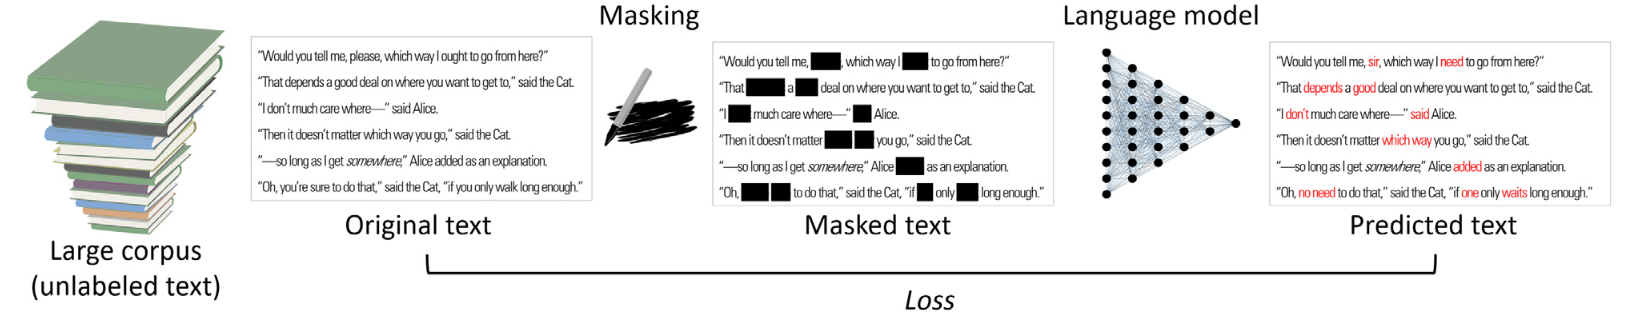
\includegraphics[scale = 0.375]{ofer_cropped.png}
    \caption{Demonstration of a self-supervised masked language learning model. A fraction of the unlabeled text is masked randomly and the language model will attempt to predict these masked tokens. The loss function is a method to asses the performance of the model on its predictions}
    \label{fig:ofer}
\end{figure}

These deep learning methods also show promise in the field of protein biology with the most notable latest projects being TAPE~\cite{tape}, ProtTrans~\cite{prottrans} and Meta AI's ESM-2~\cite{esm2}, one of the most recent and largest protein language models to ever have been developed at the time of writing. ESM-2 has shown to accurately capture evolutionary information and to perform well on structure prediction tasks. It consists of transformer protein language models with up to 15 billion parameters trained on 65 million unique sequences. Like with natural language models, it has been observed that larger models yield consistent improvement and that the performance does not seems to saturate with even the largest models~\cite{Ofer}. The amount of computing power needed to train such models and to perform predictions with them rises exponentially with the number of parameters, close to the point that modern computers cannot sustainably handle anymore. For example, it is estimated that it would take at least 34 days with 1024 NVIDIA A100 GPUs to train the 175 billion parameter GPT-3 model with 300 billion tokens~\cite{gptrain}. And although, these developments in computational modeling are very impressive, they are very costly too and cause a substantial strain on our environment in terms of the energy and materials needed to sustain these systems.